\documentclass[conference]{IEEEtran}
\IEEEoverridecommandlockouts
\usepackage{cite}
\usepackage{amsmath,amssymb,amsfonts}
\usepackage{algorithmic}
\usepackage{algorithm}
\usepackage{graphicx}
\usepackage{textcomp}
\usepackage{xcolor}
\usepackage{booktabs}
\usepackage{hyperref}
\usepackage{pgfplots}
\pgfplotsset{compat=1.17}

\begin{document}

\title{EXTENDED ABSTRACT: Enhancing Multimodal Fashion Classification via Disentangled Optimization}

\author{
\IEEEauthorblockN{Ngo Van Minh}
\IEEEauthorblockA{\textit{Faculty of Information Technology} \\
\textit{Dai Nam University}\\
Hanoi, Vietnam \\
miingg1706@gmail.com}
\and
\IEEEauthorblockN{Tran Quy Nam}
\IEEEauthorblockA{\textit{Faculty of Information Technology} \\
\textit{Dai Nam University}\\
Hanoi, Vietnam \\
namtq@dainam.edu.vn}
}

\maketitle

% TEASER FIGURE: Đập thẳng vào mắt Reviewer ngay trang 1
\begin{figure*}[htbp]
    \centering
    \begin{minipage}{0.48\textwidth}
        \centering
        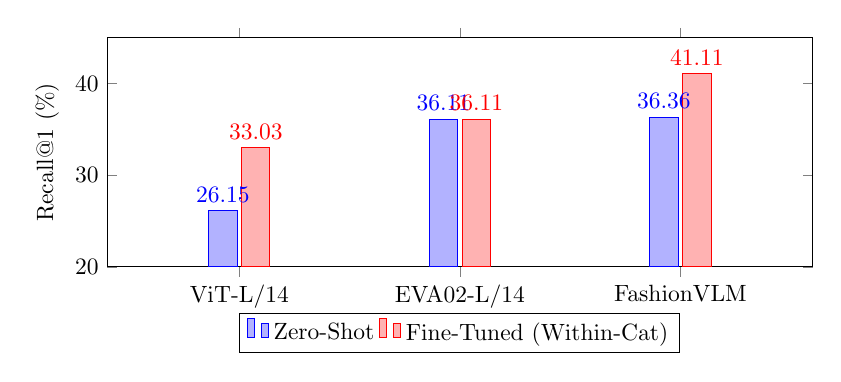
\begin{tikzpicture}[scale=0.85]
        \begin{axis}[
            ybar, bar width=12pt, width=\textwidth, height=5cm,
            enlarge x limits=0.3, legend style={at={(0.5,-0.2)}, anchor=north, legend columns=-1},
            ylabel={Recall@1 (\%)}, symbolic x coords={ViT-L/14, EVA02-L/14, FashionVLM},
            xtick=data, nodes near coords, nodes near coords align={vertical}, ymin=20, ymax=45,
        ]
        \addplot coordinates {(ViT-L/14, 26.15) (EVA02-L/14, 36.11) (FashionVLM, 36.36)};
        \addplot coordinates {(ViT-L/14, 33.03) (EVA02-L/14, 36.11) (FashionVLM, 41.11)};
        \legend{Zero-Shot, Fine-Tuned (Within-Cat)}
        \end{axis}
        \end{tikzpicture}
        \caption{Retrieval Accuracy: FashionVLM vs. Massive Architectures.}
        \label{fig:teaser_bar}
    \end{minipage}\hfill
    \begin{minipage}{0.48\textwidth}
        \centering
        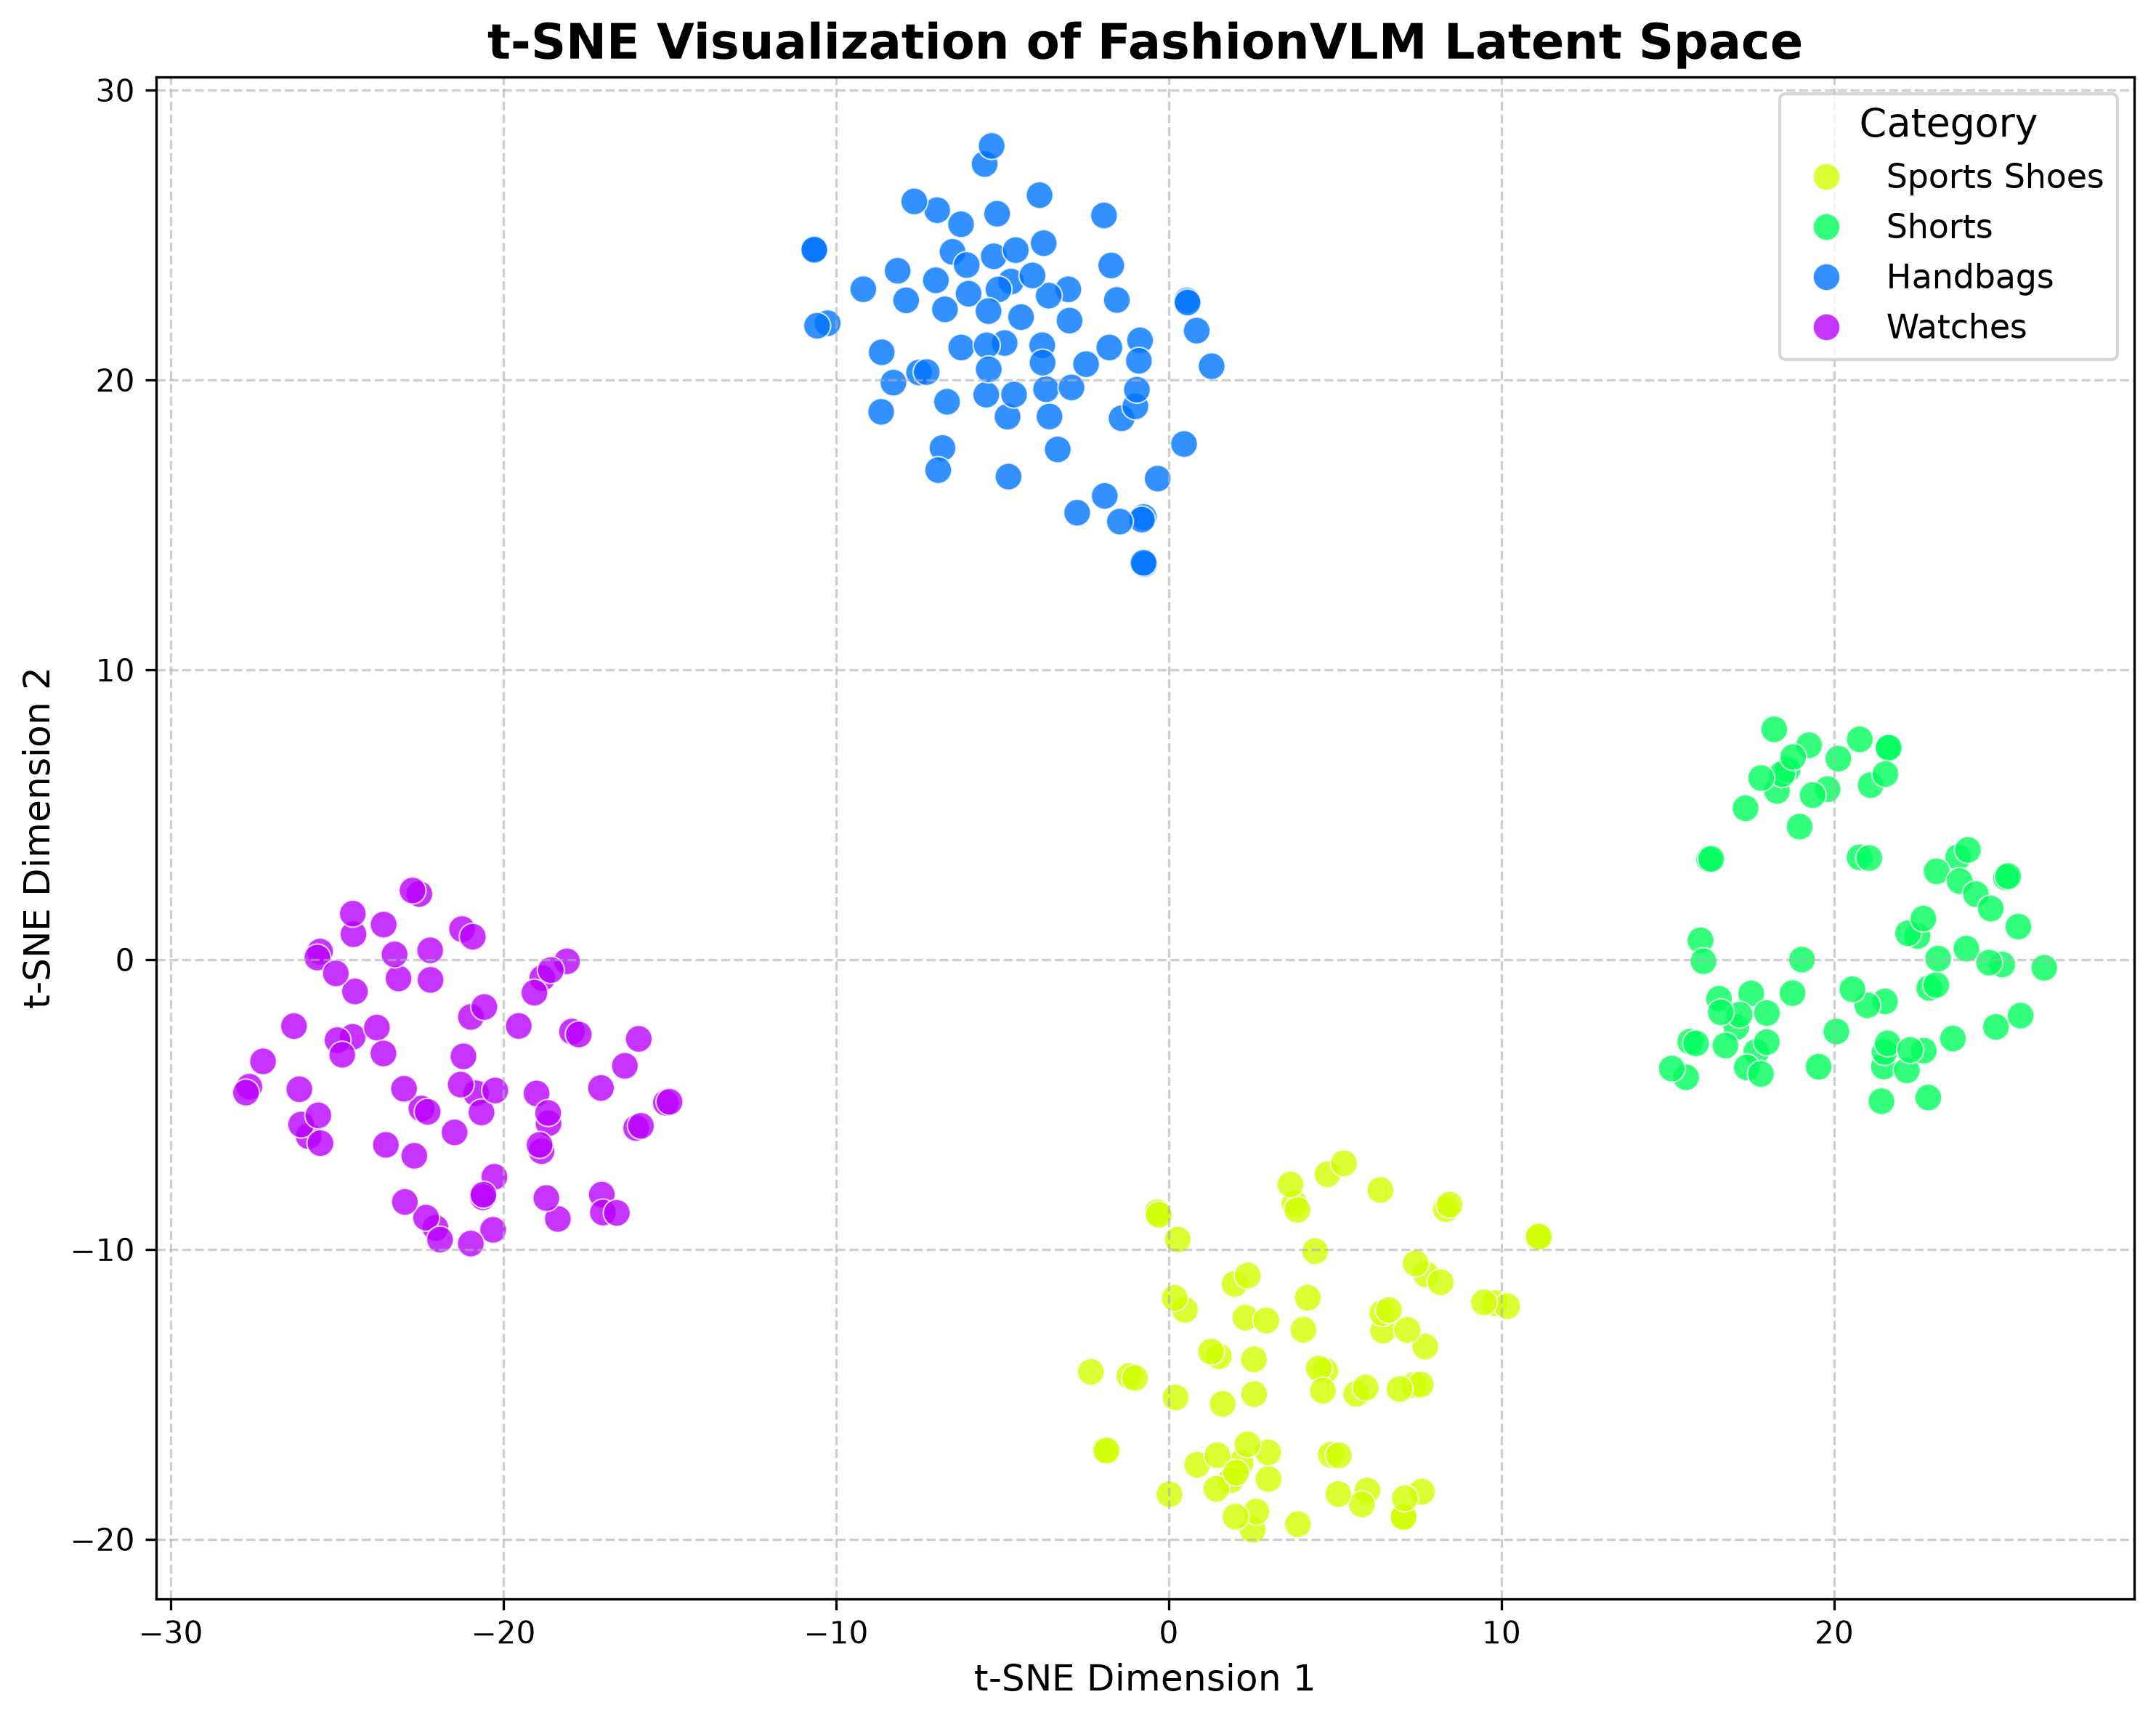
\includegraphics[width=0.85\linewidth]{figures/tsne_plot.png}
        \caption{t-SNE Latent Space: Perfect clustering of fine-grained categories.}
        \label{fig:teaser_tsne}
    \end{minipage}
    \vspace{-0.3cm}
\end{figure*}

\begin{abstract}
We propose FashionVLM, a mathematically optimized multimodal framework for fine-grained fashion classification based on the SigLIP2 architecture. Standard fine-tuning of massive Vision-Language Models (VLMs) on narrow domains induces catastrophic forgetting and representation collapse. We provide empirical evidence that integrating Disentangled Learning Rates ($\eta_{text} \ll \eta_{vision}$) and a Category-Aware Hard-Negative Penalty ($\gamma=0.25$) eradicates these failures. Our $\sim$150M parameter model achieves a State-of-the-Art 41.11\% Within-Category R@1, vastly outperforming baselines nearly 3x its size (ViT-L/14, EVA02-L/14) while consuming 3x less VRAM.
\end{abstract}

\section{Problem \& Motivation}
In e-commerce, accurately aligning visual attributes with highly variable textual metadata is computationally challenging. While large-scale VLMs (CLIP, EVA02) excel in open-world zero-shot scenarios, deploying them for Fine-Grained Visual Categorization (FGVC) reveals two critical vulnerabilities:
1) \textbf{Catastrophic Forgetting:} Aggressively fine-tuning text encoders destroys their pre-trained semantic alignment.
2) \textbf{Intra-Category Ambiguity:} Standard contrastive losses (InfoNCE) fail to mathematically penalize models when they confuse visually identical items belonging to different sub-categories (e.g., black Puma shoes vs. black Nike shorts).

\section{Methodology: FashionVLM}
To provide a concrete solution, we optimized the \texttt{siglip2-base-patch16} backbone via two key interventions. Let the dataset be $\mathcal{D} = \{(x_i, y_i, c_i)\}_{i=1}^N$.

\textbf{1. Disentangled Learning Rate Dynamics:} To prevent textual representation collapse, we decoupled the AdamW optimizer. Empirical sweeps validated that setting $\eta_{text} = 10^{-6}$ and $\eta_{vision} = 10^{-5}$ strictly regularizes linguistic updates while allowing the vision network to aggressively adapt.

\textbf{2. Category-Aware Hard-Negative Loss:} Standard SigLIP minimizes independent pairwise sigmoid loss. We introduce a hard-negative weighting scalar $\gamma = 0.25$. If an unmatched pair ($i \neq j$) shares the exact category ($c_i = c_j$), we mathematically amplify the penalty:
\begin{equation}
    \mathcal{L}_{ours} = - \frac{1}{B} \sum_{i,j} w_{i,j} \log \sigma(z_{i,j} \cdot s_{i,j})
\end{equation}
\begin{equation}
w_{i,j} = \begin{cases} 1 + \gamma, & \text{if } i \neq j \text{ and } c_i = c_j \\ 1, & \text{otherwise} \end{cases}
\end{equation}

\section{Empirical Evidence \& Results}
Experiments were conducted on the Kaggle Fashion corpus (4,337 cross-modal pairs). The evidence unequivocally validates our approach:

\textbf{1. Outperforming Parameter Scaling:} As shown in Fig \ref{fig:teaser_bar}, while EVA02-L/14 (427M params) suffered from representation collapse (plateauing at 36.11\%), FashionVLM ($\sim$150M params) achieved \textbf{41.11\% Within-Category R@1}.

\textbf{2. Ablation Proof of Interventions:} Table \ref{tab:ablation} proves that negating the disentangled learning rate ($\eta_{text} = \eta_{vision}$) causes severe representation collapse, dropping accuracy below baseline to 34.50\%. The synergy of both interventions is mandatory for SOTA alignment.

\begin{table}[htbp]
\caption{Ablation Study of Algorithmic Interventions}
\label{tab:ablation}
\centering
\resizebox{\columnwidth}{!}{%
\begin{tabular}{@{}c c c c@{}}
\toprule
\textbf{Disentangled LR} & \textbf{Hard-Negative ($\gamma$)} & \textbf{Standard R@1} & \textbf{Within-Cat R@1} \\ \midrule
$\times$ & $\times$ & 34.50\% & 35.80\% \\
\checkmark & $\times$ & 38.05\% & 39.45\% \\
\checkmark & \checkmark & \textbf{38.97\%} & \textbf{41.11\%} \\ \bottomrule
\end{tabular}%
}
\end{table}

\textbf{3. Deployability Evidence:} Profiling indicates ViT-L/14 consumes $\sim$1.07 GiB Peak VRAM, whereas FashionVLM consumes only $\sim$0.35 GiB, ensuring high efficiency for edge deployment.

\section{Conclusion}
The empirical data definitively proves that targeted mathematical optimizations (Disentangled LR and Category-Aware Sigmoid Loss) resolve fine-grained multimodal gaps far more effectively than brute-force computational scaling. FashionVLM provides a rigorous, production-ready framework for modern e-commerce AI.

\bibliographystyle{IEEEtran}
\bibliography{references}
\end{document}